\section{Мета роботи}
Набути навичок та закріпити знання при виконанні операцій пошуку.
\\

\noindent
\textbf{Теми для попередньої роботи:}
\begin{itemize}
    \item набори даних: масиви, лінійні списки;
    \item алгоритми пошуку за числовомим ключом: лінійний, лінійний з бар’єром, двійковий, експоненційний, інтерполяційний;
    \item алгоритми пошуку зразка в тексті: прямий, КМП, БМ алгоритми.
\end{itemize}


\section{Завдання}
Розробити та налагодити програму, в якій реалізувати два алгоритми
пошуку відповідно до завдання. Порівняти алгоритми за часом роботи.

На етапі тестування для кожного з алгоритмів (варіанти 4 – 15)
визначити кількість порівнянь у наборі даних з різною кількістю елементів
(20, 100, 1000, 10000) визначити час пошуку, заповнити таблицю за формою
табл. 9.1, побудувати графіки, зробити висновки. При роботі з текстом
(варіанти 1 – 3) змінювати довжину текста та зразка.

УВАГА! У завданнях 4 – 15 передбачена робота з цілими числами;
наступні 12 завдань (номери 16 – 27) вимагають роботу з дійсними числами.

\noindent
\textbf{Завдання за варіантом (\variant): }Двійковий та лінійний пошуки у лінійному списку.


\section{Хід виконання}
Для виконання завдання було обрано мову Rust.
Увесь код також додатково був розміщений в GitHub репозитарії: \href{https://github.com/blackgolyb/algos-labs}{https://github.com/blackgolyb/algos-labs}.


\newpage
\subsection{Лінійний пошук}
\lstinputlisting[language=Rust, style=colouredRust]{\codeDirectory/src/labs/lab9/variants/linear.rs}


\newpage
\subsection{Двійковий пошук}
\lstinputlisting[language=Rust, style=colouredRust]{\codeDirectory/src/labs/lab9/variants/binary.rs}


\newpage
\subsection{Приклад роботи програми}
Для перевірки працездатності напишемо програму яка буде порівнювати двійковий та лінійний пошук у лінійному списку.
Порівнювати будемо за такими критеріями:
кількість порівнянь, кількість переходів до наступного вузла та час пошуку.


\noindent
Код програми для перевірки:
\lstinputlisting[language=Rust, style=colouredRust]{\codeDirectory/src/labs/lab9/main.rs}


\begin{figure}[ht!]
    \centering
    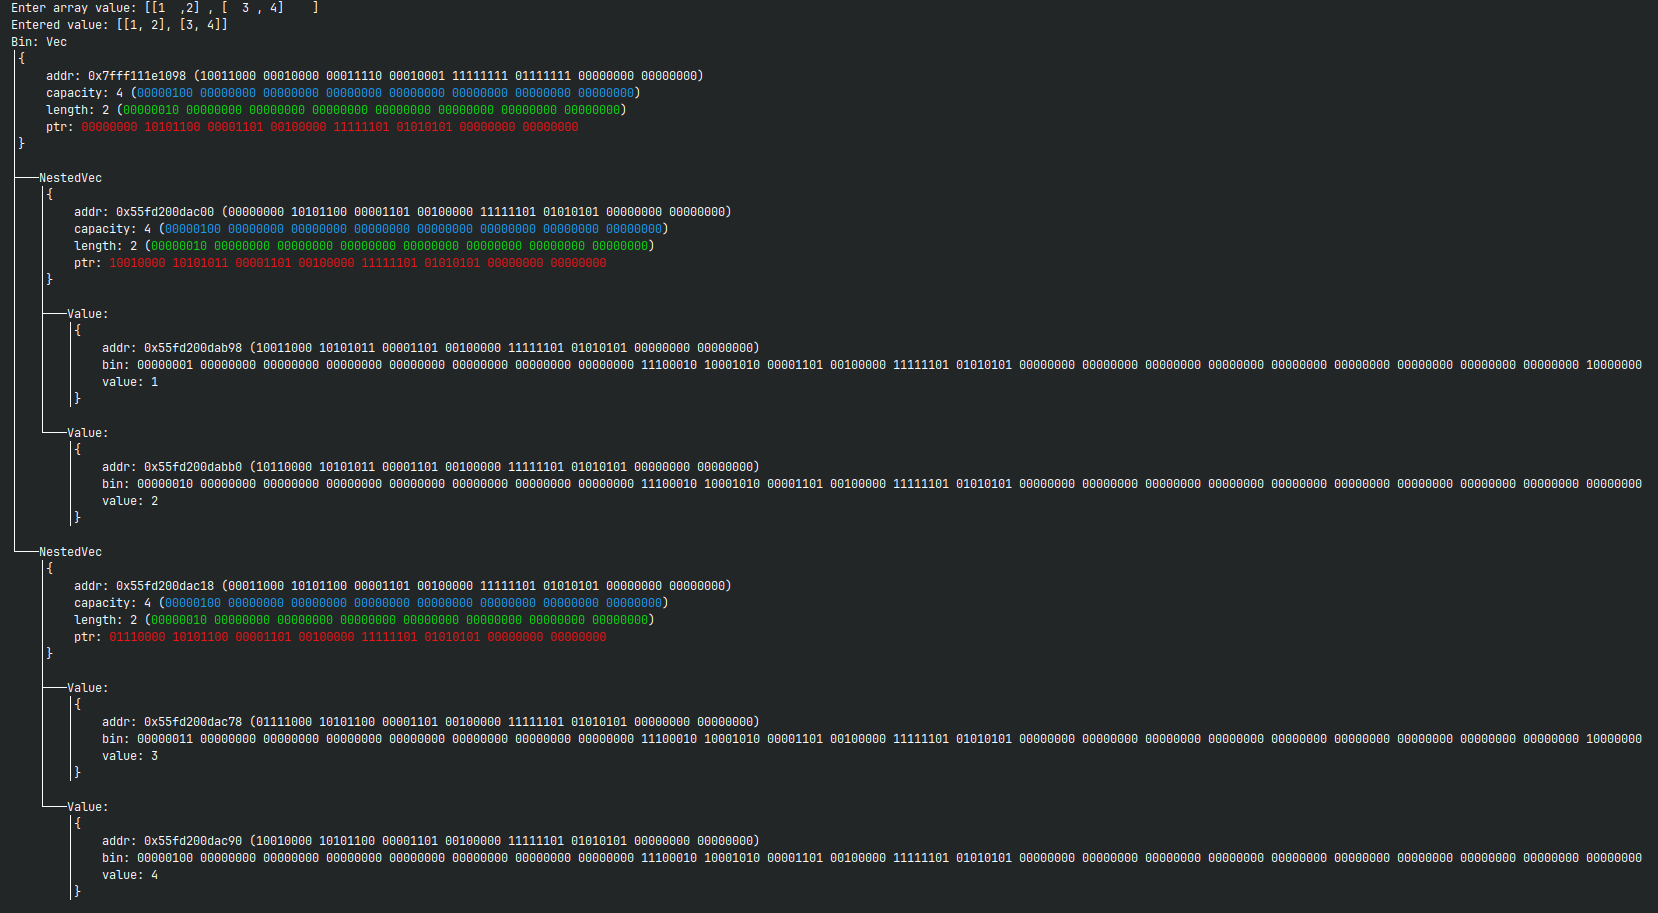
\includegraphics[width=.8\textwidth]{\assetsDirectory/res.png}
    \caption{Приклад роботи}
\end{figure}

\begin{figure}[ht!]
    \centering
    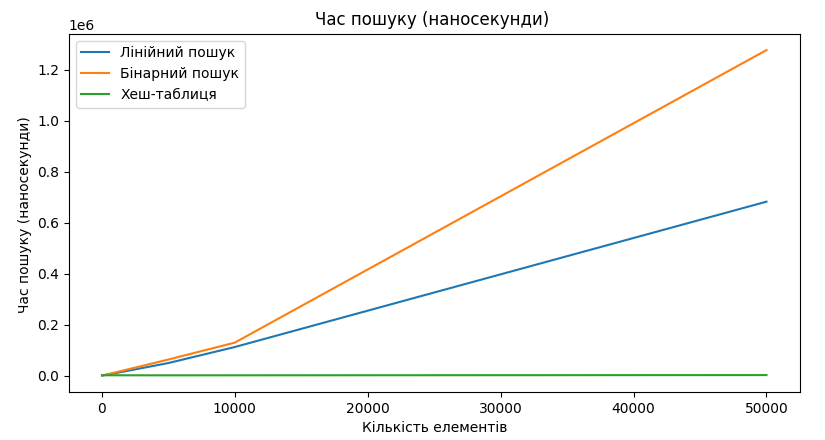
\includegraphics[width=.8\textwidth]{\assetsDirectory/time.png}
    \caption{Залежність часу пошуку від кількості елементів}
\end{figure}
\begin{figure}[ht!]
    \centering
    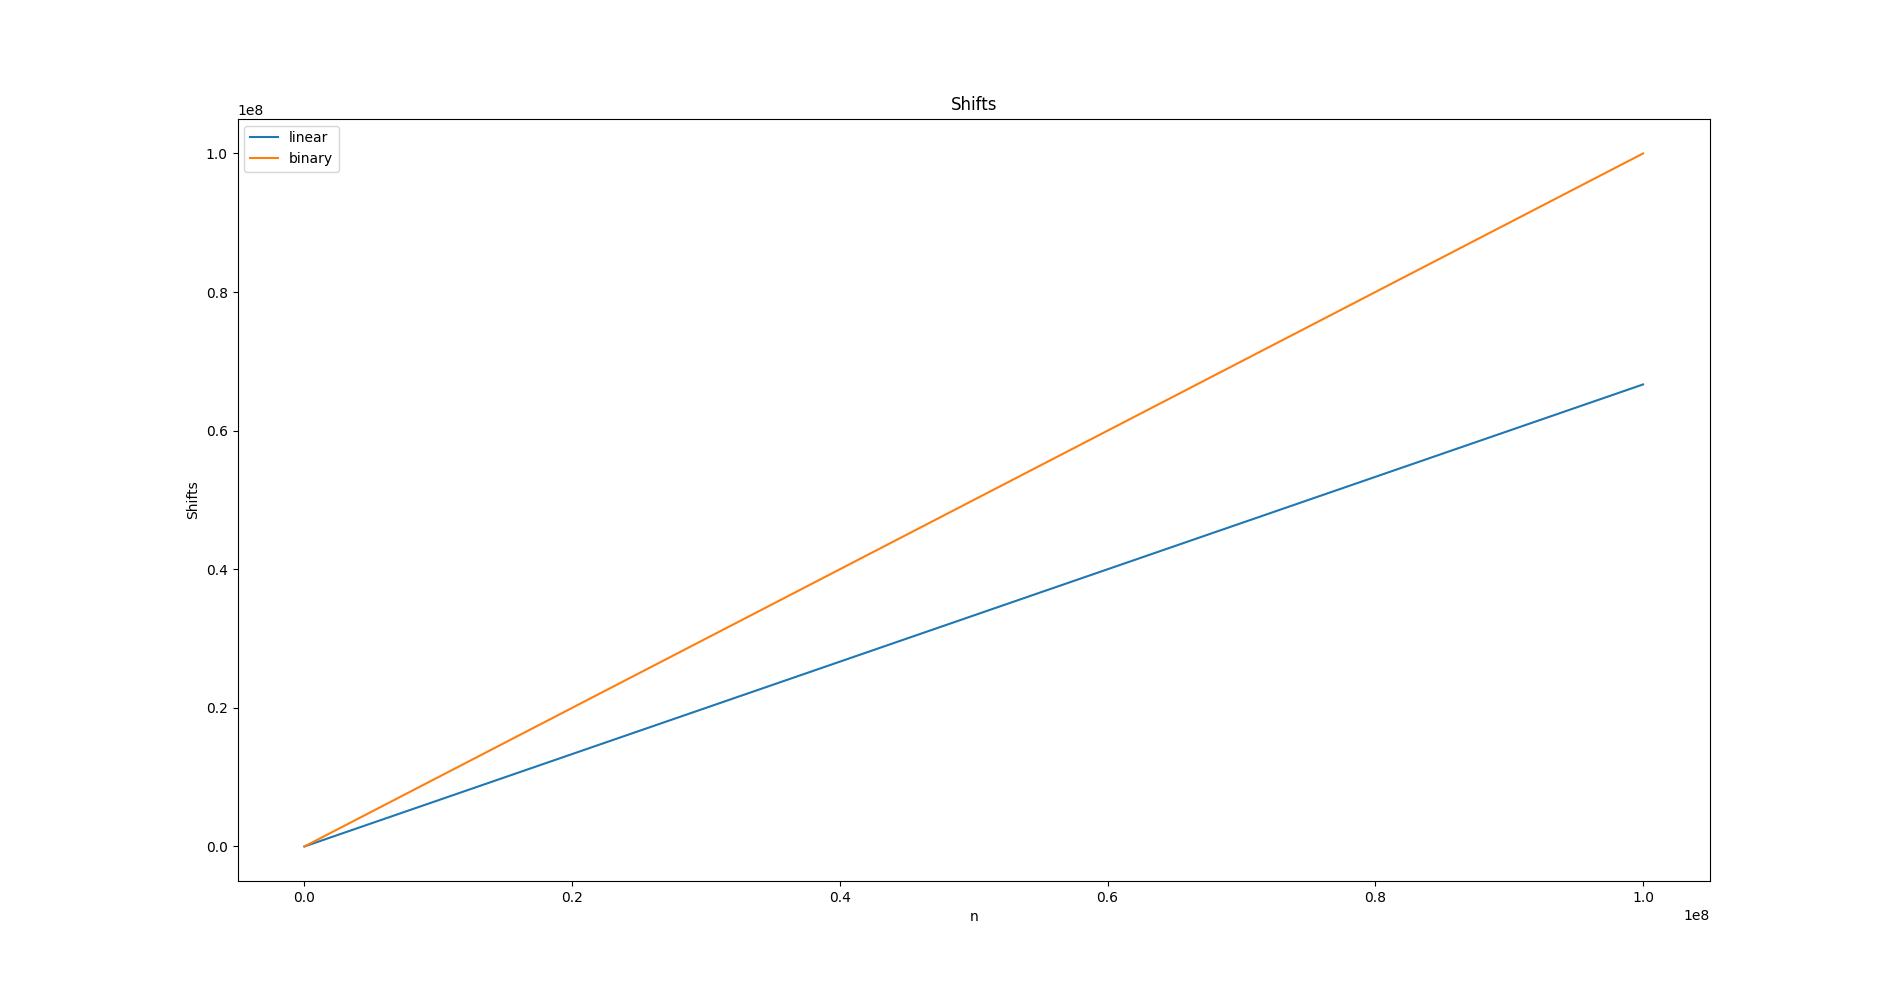
\includegraphics[width=.8\textwidth]{\assetsDirectory/shift.png}
    \caption{Залежність переходів до наступного вузла від кількості елементів}
\end{figure}
\begin{figure}[ht!]
    \centering
    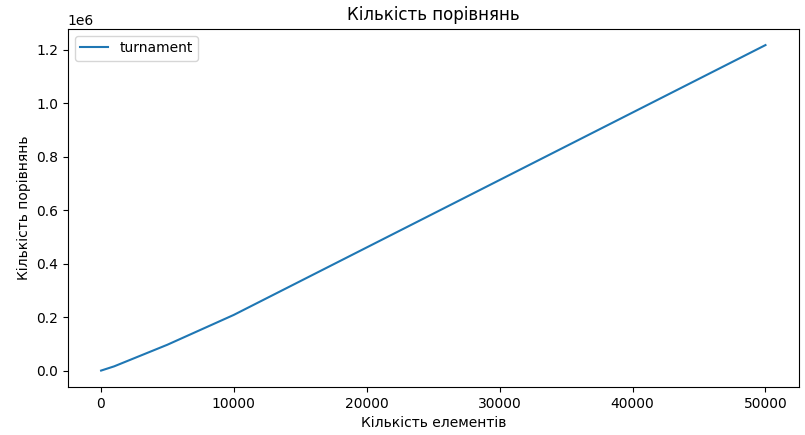
\includegraphics[width=.8\textwidth]{\assetsDirectory/comp.png}
    \caption{Залежність кількості порівнянь від кількості елементів}
\end{figure}


\newpage
\section{Висновки}
В ході виконання лабораторної робити було створено лінійний та бінарний пошук у лінійному списку.
За результатами порівняння було виявлено, що лінійний пошук займає менше часу і менше кількості переходів до наступного вузла,
проте робить набагато більше порівнянь.
Бінарний пошук займає більше часу і більше переходів до наступного вузла, але виконує менше порівнянь.
Також явно прослідковується кореляція часу та переходів до наступного вузла,
а внесок меншої кількості порівнянь не значно впливає на час всього пошуку.
Що є логічним, бо операція порівняння цілих чисел значно швидша за операцію разадресації яка виконується при кожному переході до наступного вузла.
Тому за умови що операція разадресації на порядок довша за порівняння, тоді лінійний пошук буде кращім рішенням для зв'язного списку.
